\section*{Assignment 3}
% Ampel
% 3 FPGA's 2 with ampel the other as Translator 
% at 1st only the 2 ampels, watching with oszyluscope how they communicate.
% at 2nd communicating with on ampel though the fpga transmitting asci keys to imitate the 2nd ampel
% 3rd Man in the middle

% 3modes both green
% both red
% normal working

% See figure \ref{fig:as3-schematic} (p.~\pageref{fig:as3-schematic}).

Two identically programmed micro controllers, equipped with three different-colored LEDs (red, yellow and green) and communicating via UART, are handed to us. 
In operation only one of the lights is active at a time per device. 
While one device's red LED is active, the other device's green one is illuminated. 
After some time the green light turns to yellow and then to red, causing the first device to activate the green light -- they resemble two simple traffic lights. 

In a first step we are asked to reverse engineer the underlying protocol. 
To do so, we hook an oscilloscope to the \texttt{rx} and \texttt{tx} lines of one device and observe its behavior during and after a reset. 
We see the red light active and one single ASCII byte $47_{16}$, `G', being transmitted. 
We conjecture that  whenever one micro controller finishes transitioning from showing the green light to showing the red light, it sends out `G' to signal the other device that it is safe to turn to green. 
We test our hypothesis by connecting one micro controller directly to the computer and in case that we send the letter `G', it instantly illuminates the green light and transitions to showing the red light soon after, staying like this if we do not interact further.

Now we are ready for the real assignment: To launch a man-in-the-middle attack against the traffic lights protocol, implementing the three following modes of operation.

\begin{itemize}
    \item[] \begin{labeling}{\textsf{Throughput}$^1$:}
        \item[\textsf{Throughput}\footnotemark:] the FPGA passively relays the communication between the devices like a cable (the default setting);
        \item[\textsf{Green}:] manipulate the communication in a way that both micro controllers constantly show the green light;
        \item[\textsf{Red}:] after cutting the communication links to the devices, both will display the red light (this can lead to starvation because `G' is only sent once when activating the red light).
    \end{labeling}
    \footnotetext[1]{Actually the correct term would be `pass through', but since we used the wrong one throughout the lab days, we are sticking to `throughput'.}
\end{itemize}


As a side requirement we should to be able to cycle through the modes seamlessly, i.~e., no matter which mode $M$ the FPGA is in, we can always choose the next one $M'$ freely.

We start with \textsf{Throughput} by connecting the \texttt{tx} line of one device to the \texttt{rx} line of the other and vice versa, passing the signals directly through the FPGA. 
Next, we add a receiver to get commands from the computer and use a simple feedback loop to report them back. 
To implement \textsf{Green}, we have to send `G' continuously to both devices, therefore we include a transmitter with constant input byte `G', which is always enabled.
Finally, \textsf{Red} just outputs the static UART idle bit, $1_2$, to the micro controllers. 
Multiplexers are used to select the correct output signals corresponding to each mode. 

\begin{figure}[tb]
    \begin{center}
        \usetikzlibrary{arrows.meta}
\usetikzlibrary{calc,intersections,through,backgrounds}
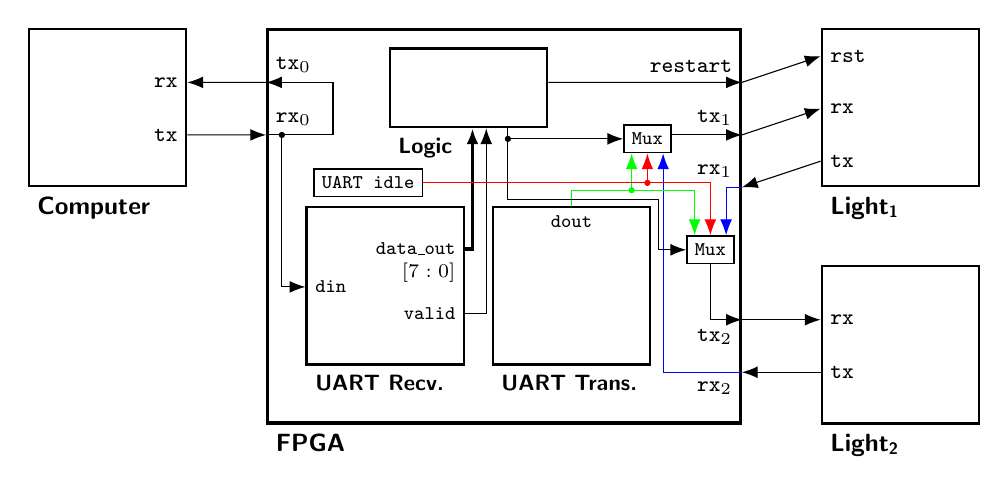
\begin{tikzpicture}
	\tikzset{comp/.style={
		rectangle, draw=black, thick
	}}	
	\tikzset{component/.style={
		comp, minimum width=6cm, minimum height=5cm, very thick
	}}
	\tikzset{component_small/.style={
		comp, minimum width=2cm, minimum height=2cm, thick
	}}
	\tikzset{component_tiny/.style={
		comp, inner sep=0.1cm, semithick
	}}
	\tikzset{caption/.style={
		below right
	}}
	\tikzset{conn/.style={
		-{Latex[length=2mm]}
	}}
	
	% FPGA
	\node (FPGA) [component] at (0,0) {}
		% Caption
		node [caption] at (FPGA.south west) { \small{\textsf{\textbf{FPGA}}} }
		
		% In/-outputs links
		coordinate [yshift=3cm+0.4pt+0.666cm, label={ above right : \footnotesize{$\texttt{rx}_0$} }] (FPGA_rx0) at (FPGA.south west) % unten
		coordinate [yshift=3cm+0.4pt+1.333cm, label={ above right : \footnotesize{$\texttt{tx}_0$} }] (FPGA_tx0) at (FPGA.south west) % oben

		% In/outputs  rechts oben
		coordinate [yshift=3cm+0.4pt,                    label={ above left : \footnotesize{$\texttt{rx}_1$} }]      (FPGA_rx1)       at (FPGA.south east)  % unten
		coordinate [yshift=3cm+0.4pt+0.666cm, label={ above left : \footnotesize{$\texttt{tx}_1$} }]      (FPGA_tx1)       at (FPGA.south east) % mitte
		coordinate [yshift=3cm+0.4pt+1.333cm, label={ above left : \footnotesize{$\texttt{restart}$} }] (FPGA_restart) at (FPGA.south east) % oben
		
		% In/outputs  rechts unten
		coordinate [yshift=0.666cm,           label={ below left : \footnotesize{$\texttt{rx}_2$} }]      (FPGA_rx2)        at (FPGA.south east)  % unten
		coordinate [yshift=1.333cm,           label={ below left : \footnotesize{$\texttt{tx}_2$} }]      (FPGA_tx2)        at (FPGA.south east) % oben

		% Interna
		node (UART_idle) [component_tiny, shift={(-1.725cm, 0.55cm)}] at (FPGA)           { \scriptsize{\textsf{\texttt{UART idle}}} }
	 	node (Mux1)          [component_tiny, shift={(-1.2cm, -0.05cm)}]  at (FPGA_tx1)   { \scriptsize{\textsf{\texttt{Mux}}} }
	 	node (Mux2)          [component_tiny, shift={(-0.4cm, -0.3cm)}]    at (FPGA.east) { \scriptsize{\textsf{\texttt{Mux}}} }
	;

	% Logic
	\node (Logic) at (FPGA.north) [comp, minimum height=1cm, minimum width=2cm, below, shift={(-0.45cm, -0.25cm)}] {}
		node [caption] at (Logic.south west) { \textsf{\footnotesize{\textbf{Logic}}} }
	;

	% Receiver
	\node (Receiver) at (FPGA.south west) [component_small, above right, shift={(0.5, 0.75)}] {}
		% Caption
		node [caption] at (Receiver.south west) { \textsf{\footnotesize{\textbf{UART Recv.}}} }

		% Input links
		coordinate [yshift=1cm, label={ right : \scriptsize{\texttt{din}} }] (Receiver_din) at (Receiver.south west)

		% Outpus links
		coordinate [yshift=0.666cm,                 label={ left : \scriptsize{\texttt{valid}} }]           (Receiver_valid)           at (Receiver.south east) % unten
		coordinate [yshift=1.333cm+0.15cm, label={ left : \scriptsize{\texttt{data\_out}} }] (Receiver_data_out)    at (Receiver.south east) % oben
		coordinate [yshift=1.333cm-0.15cm,  label={ left : \scriptsize{$[7:0]$} }]                     (Receiver_data_out2) at (Receiver.south east) % mitte
	;

	% Transmitter
	\node (Transmitter) at (FPGA.south east) [component_small, above left, shift={(-1.15, 0.75)}] {}
		node [caption] at (Transmitter.south west) { \textsf{\footnotesize{\textbf{UART Trans.}}} }

		% Output oben
		coordinate [label={ below : \scriptsize{\textsf{\texttt{dout}}} }] (Transmitter_dout) at (Transmitter.north) % unten
	;

	% Computer
	\node (Computer) [component_small, below left, xshift=-1cm] at (FPGA.north west) {}
		% Caption
		node [caption] at (Computer.south west) { \small{\textsf{\textbf{Computer}}} }

		% In/outputs rechts
		coordinate [yshift=0.666cm, label={ left:\footnotesize{\texttt{tx}} }] (Computer_tx) at (Computer.south east) % unten
		coordinate [yshift=1.333cm, label={ left:\footnotesize{\texttt{rx}} }] (Computer_rx) at (Computer.south east) % oben
	;

	% Light 1
	\node (Light_1) [component_small, below right, xshift=1cm] at (FPGA.north east) {}
		% Caption
		node [caption] at (Light_1.south west) { \small{\textsf{\textbf{Light\textsubscript{1}}}} }

		% In/outputs links
		coordinate [yshift=0.333cm, label={ right:\footnotesize{\texttt{tx}} }]   (Light_1_tx)   at (Light_1.south west) % unten
		coordinate [yshift=0.999cm, label={ right:\footnotesize{\texttt{rx}} }]   (Light_1_rx)   at (Light_1.south west) % mitte
		coordinate [yshift=1.666cm, label={ right:\footnotesize{\texttt{rst}} }] (Light_1_rst) at (Light_1.south west) % oben
	;

	% Light_2
	\node (Light_2) [component_small, above right, xshift=1cm] at (FPGA.south east) {}
		% Caption
		node [caption] at (Light_2.south west) { \small{\textsf{\textbf{Light\textsubscript{2}}}} }

		% In/outputs links
		coordinate [yshift=0.666cm, label={ right:\footnotesize{\texttt{tx}} }]   (Light_2_tx)   at (Light_2.south west) % unten
		coordinate [yshift=1.333cm, label={ right:\footnotesize{\texttt{rx}} }]   (Light_2_rx)   at (Light_2.south west) % oben
	;

	% Computer <-> FPGA
	\draw[conn]  (FPGA_tx0) -- (Computer_rx);
	\draw[conn] (Computer_tx) -- (FPGA_rx0);
	
	% FPGA <-> Lights
	\draw[conn] (FPGA_restart) -- (Light_1_rst);
	\draw[conn] (FPGA_tx1) -- (Light_1_rx);
	\draw[conn] (Light_1_tx) -- (FPGA_rx1) ;
	\draw[conn] (FPGA_tx2) -- (Light_2_rx);
	\draw[conn] (Light_2_tx) -- (FPGA_rx2);
	
	% FPGA internal
		\draw[conn] ([yshift=0.583cm] Logic.south east) -- (FPGA_restart); % logic -> restart
		\draw[conn, name path=FPGA_rx0--FPGA_tx0] (FPGA_rx0) -- ([xshift=0.85cm] FPGA_rx0) |- (FPGA_tx0); % Computer input feedback loop

		% Connections to/from Receiver
	 	\draw[conn, name path=FPGA_rx0--Receiver_din] (FPGA_rx0) -- ([xshift=0.2cm] FPGA_rx0)  |- (Receiver_din); % tx0 -> receiver
		\draw[conn, very thick] (Receiver_data_out) -| ([xshift=0.05cm] Logic.south);  % receiver -> logic
		\draw[conn] (Receiver_valid) -|  ([xshift=0.225cm] Logic.south); % receiver -> logic

		% Connections to/from Mux1
		\draw[conn, name path=Logic--Mux1] ([xshift=0.5cm] Logic.south) |- (Mux1.west);
		\draw[conn, draw=red, name path=UART_idle--Mux1] (UART_idle) -| (Mux1); % UART_idle -> Mux1	
		\draw[conn, color=green, name path=Transmitter_dout--Mux1] (Transmitter_dout) -- ([yshift=0.2cm] Transmitter_dout) -| ([xshift=-0.2cm] Mux1.south); % dout -> Mux1
		\draw[conn, color=blue] (FPGA_rx2) -| ([xshift=0.2cm] Mux1.south); % rx2 -> Mux1
		\draw[conn, yshift=0.5cm] ([yshift=0.05cm] Mux1.east) -- (FPGA_tx1); % Mux1 -> tx1

		% Connections to/from Mux2
		\draw[conn, name path=Logic--Mux2] ([xshift=0.5cm] Logic.south) -- ([shift={(0.5cm, -0.9cm)}] Logic.south) -| ([xshift=-0.35cm] Mux2.west) -- (Mux2.west);
		\draw[conn, draw=red, name path=UART_idle--Mux2] (UART_idle) -| (Mux2); % UART_idle -> Mux2
		\draw[conn, draw=green, name path=Transmitter_dout--Mux2] ([yshift=0.2cm] Transmitter_dout) -| ([xshift=-0.2cm] Mux2.north); % dout -> Mux2
		\draw[conn, draw=blue] (FPGA_rx1) -| ([xshift=0.2cm] Mux2.north);	 % rx1 -> Mux2
		\draw[conn] (Mux2) |- (FPGA_tx2); % Mux2 -> tx2
		
		% Intersections
		\fill[name intersections={of=FPGA_rx0--FPGA_tx0 and FPGA_rx0--Receiver_din, total=\t}] (intersection-\t) circle (0.4mm);
		\fill[name intersections={of=Logic--Mux1 and Logic--Mux2, total=\t}] (intersection-\t) circle (0.4mm);
		\fill[red, name intersections={of=UART_idle--Mux1 and UART_idle--Mux2, total=\t}] (intersection-\t) circle (0.4mm);
		\fill[green, name intersections={of=Transmitter_dout--Mux1 and Transmitter_dout--Mux2, total=\t}] (intersection-\t) circle (0.4mm);
\end{tikzpicture}
        \caption{FPGA in the middle with three modes of operation \textsf{Throughput} (\textcolor{blue}{blue}), \textsf{Green} (\textcolor{green}{green}) and \textsf{Red} (\textcolor{red}{red}) controlled via the computer. The transmitter is always enabled and has a fixed input byte producing a cyclic bitstream \texttt{dout}. Outputs and hence operation mode are selected by multiplexers.}
        \label{fig:as3-schematic}
        \vspace{1em}\hrule
    \end{center}
\end{figure}

To tackle the starvation problem, we need to add a simple finite state machine that knows the current and next operation modes, triggering the reset signal of one device, if the FPGA is about to switch from \textsf{Red} to \textsf{Throughput} -- all other operation mode transitions already work as desired. We use a voltmeter to find the actual \texttt{rst} pin on the micro controller, by effectively short-circuiting all unconnected pins at a time [?].
